\documentclass{article}

% Language setting
% Replace `english' with e.g. `spanish' to change the document language
\usepackage[spanish]{babel}

% Set page size and margins
% Replace `letterpaper' with `a4paper' for UK/EU standard size
\usepackage[letterpaper,top=2cm,bottom=2cm,left=3cm,right=3cm,marginparwidth=1.75cm]{geometry}
% Useful packages
\usepackage{amsmath}
\usepackage{graphicx}
\usepackage[colorlinks=true, allcolors=blue]{hyperref}
\title{Informe sobre accesibilidad web}
\author{ Minerva Quintero Flores \and Andrés Felipe Vargas Cortés}

\begin{document}
\maketitle

\section{Introducción}

En el transcurso de este informe, hemos llevado a cabo un análisis de la página web principal de Nescafé y la aplicación de móvil Instagram con el propósito de evaluar su nivel de accesibilidad, basándonos en las directrices y recomendaciones establecidas por las WCAG (Web Content Accessibility Guidelines). Estas pautas son fundamentales para garantizar que los sitios web y móvil sean accesibles y utilitarios para todas las personas, incluyendo aquellas con diversas discapacidades.

Nuestra evaluación se ha centrado en examinar a través de un enfoque multidimensional, en el cual hemos considerado cuidadosamente los siguientes principios clave:

\begin{itemize}
    \item Perceptibilidad: Este principio pone énfasis en la capacidad de la página web para que la información presentada sea perceptible de manera efectiva por todos los usuarios.

    \item Operabilidad: Evaluamos la operabilidad de la página web, asegurándonos de que sea posible interactuar y navegar por ella de manera efectiva, incluso para aquellas personas que utilizan tecnologías de asistencia como lectores de pantalla. 
    \item Comprensibilidad: Hemos analizado la claridad y la simplicidad con la que se presenta la información en la página web. 
    \item Robustez: El principio de robustez se refiere a la capacidad de la página web para funcionar de manera coherente y confiable en diversos entornos y dispositivos.
\end{itemize}

Además de nuestra evaluación manual, hemos complementado este análisis con una segunda revisión que utiliza herramientas especializadas diseñadas para evaluar de forma automática la calidad y accesibilidad de la página web. En particular, hemos empleado las herramientas Google Lighthouse y Wave, que ofrecen métricas objetivas y datos detallados que respaldan nuestras conclusiones sobre la accesibilidad y el rendimiento del sitio web de Nescafé.

Este informe busca proporcionar una visión integral de la accesibilidad, ofreciendo recomendaciones y observaciones que contribuyan a mejorar la experiencia en línea para todos los usuarios, sin importar sus habilidades o capacidades.

\newpage

\section{Análisis Manual:}


\subsection{Perceptible:}

Por lo general la pagina web cumple a la hora de poner alternativas de texto, pero tiene un par de botones los cuales no tienen texto, por lo que una persona con problemas de visión no sería capaz de saber su utilidad.

\begin{figure}[!h] 
\centering
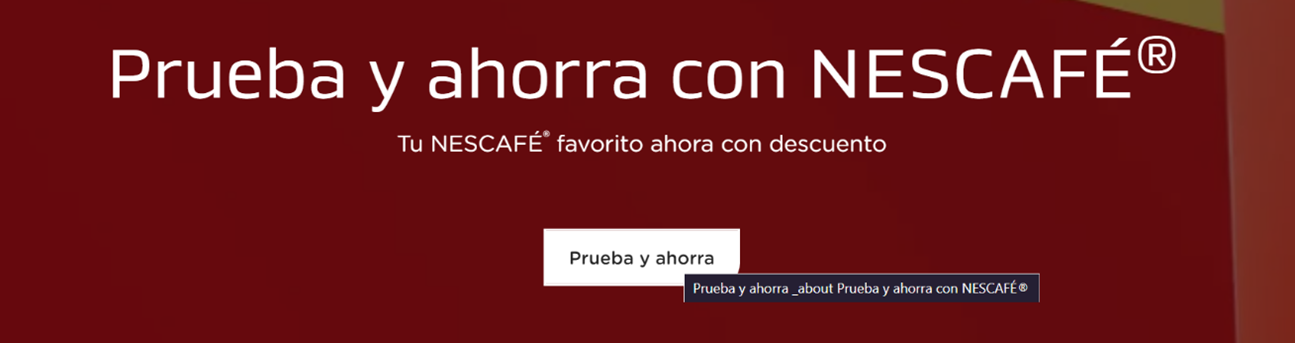
\includegraphics[width=0.5\linewidth]{Imagen1.png}
\caption{\label{fig:frog}Ejemplo con alternativa de texto.}
\end{figure}

\begin{figure}[!h] 
        \centering
        
\includegraphics[width=0.5\linewidth]{Imagen2.png}
        \caption{ Ejemplo sin alternativa de texto}
\end{figure}


\subsection{Operable:}

El área de la página web donde se encuentran la mayoría de los problemas en términos de accesibilidad es en la navegación y la interacción mediante el teclado. Se han identificado secciones específicas que no son accesibles utilizando solo el teclado como herramienta de navegación. Este problema es realmente preocupante, ya que limita significativamente la experiencia de usuario de aquellas personas que dependen de dispositivos de entrada alternativos, como lectores de pantalla o teclados especiales, debido a discapacidades motoras o condiciones que dificultan el uso del mouse.

\begin{figure}[!h]
        \centering
        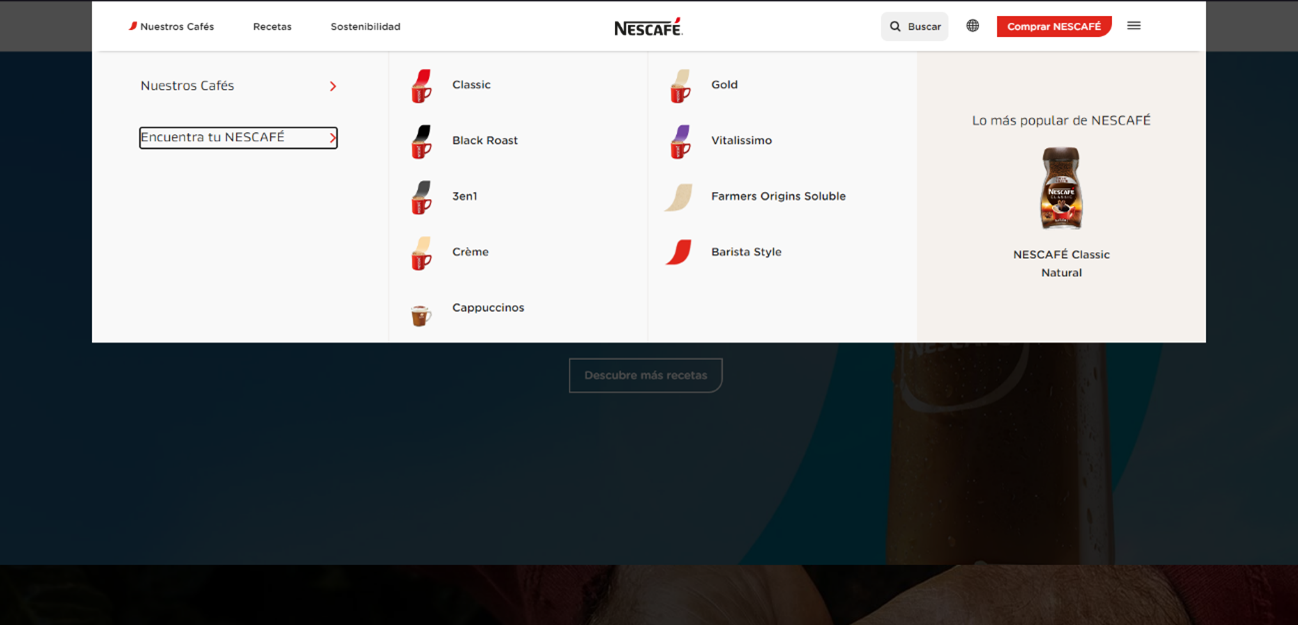
\includegraphics[width=1\linewidth]{Imagen3.png}
        \caption{Secciones inaccesibles de Nescafé}
\end{figure}

Tanto la sección de "Recetas" como "Sostenibilidad" son totalmente inaccesibles salvo que dispongas de un ratón. Lo mismo pasa con el botón “Compra aquí”, visto en el apartado anterior, no se puede llegar a el mediante teclado y este es a nuestro parecer el error mas grande de la página ya que es una de las funcionalidad principales, ya que te permite hacer la compra del producto de forma online, con este problema de accesibilidad la página se vuelve prácticamente inútil para cualquier persona con discapacidades motoras o visuales.

\begin{figure}[!h] 
\centering
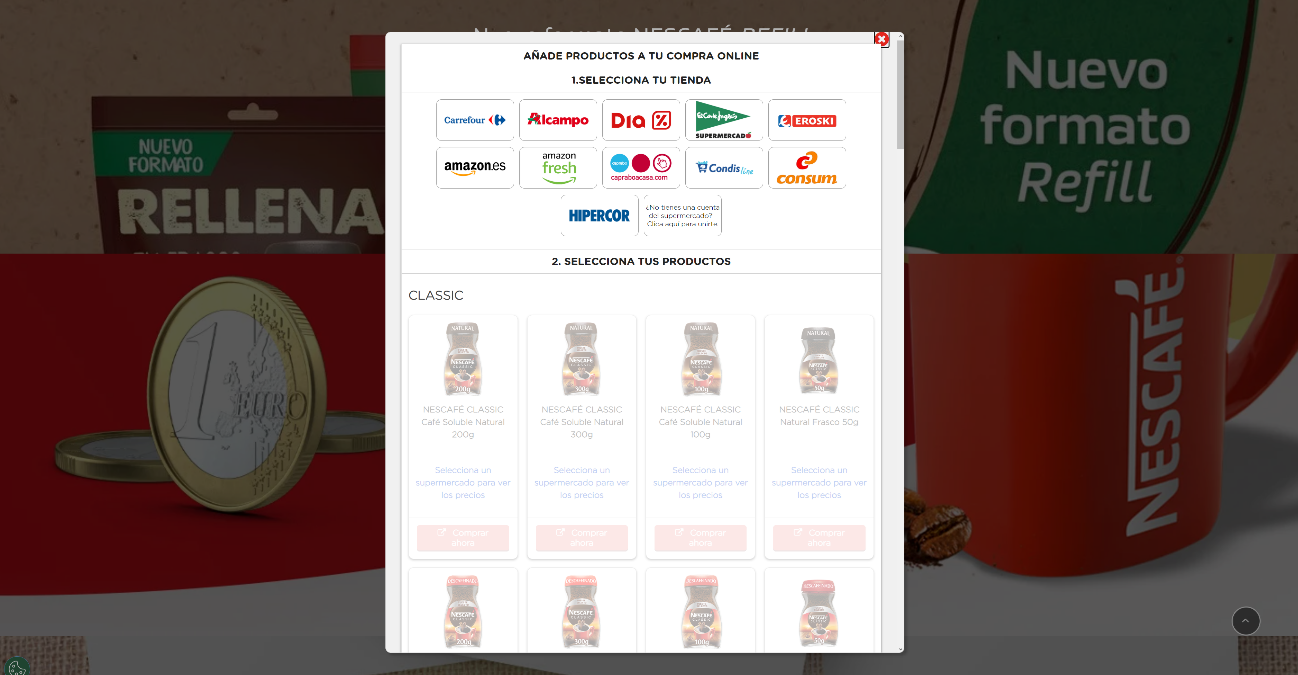
\includegraphics[width=0.5\linewidth]{Imagen4.png}
\caption{Compra Nescafé online inaccesible mediante teclado}
\end{figure}

\subsection{Comprensible:}
En líneas generales, la página web cumple satisfactoriamente con su objetivo principal de proporcionar información de manera comprensible y efectiva. Uno de sus puntos fuertes radica en la elección de paletas de colores que garantizan buenos contrastes, lo que facilita la legibilidad y la claridad visual de los contenidos. Además, la presentación de información se lleva a cabo de manera no ambigua, lo que ayuda a los usuarios a comprender de manera efectiva el contenido disponible en el sitio.

\subsection{Robusto:}

Inicialmente, la página web presenta un rendimiento aceptable en cuanto a su accesibilidad, aunque no está exenta de algunas deficiencias. Como mencionamos anteriormente, uno de los problemas identificados se refiere a la falta de descripciones adecuadas para los botones, lo que dificulta su comprensión para usuarios que dependen de lectores de texto debido a problemas de visión. Este inconveniente no solo afecta la experiencia de navegación de estas personas, sino que también limita la interacción efectiva con el contenido y las funcionalidades del sitio.

\newpage

\section{Análisis Automáticos:}

\subsection{Google lighthouse:}

Utilizamos Google Lighthouse para realizar un análisis automático de accesibilidad en el sitio web. Esta herramienta nos ayuda a identificar y abordar problemas relacionados con la accesibilidad, garantizando una experiencia inclusiva para todos los usuarios.

\begin{figure}[!h]
        \centering
        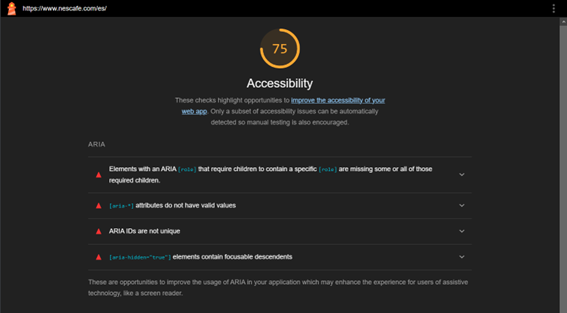
\includegraphics[width=1\linewidth]{Imagen5.png}
        \caption{Resultados análisis de www.nescafé.es}
\end{figure}


Los primeros errores que la herramienta detecta están relacionados con la robustez de la página. Estos problemas incluyen la presencia de IDs duplicados, atributos que contienen elementos no válidos y la ausencia de ciertos elementos esenciales en el código.

\begin{figure}[!h]
        \centering
        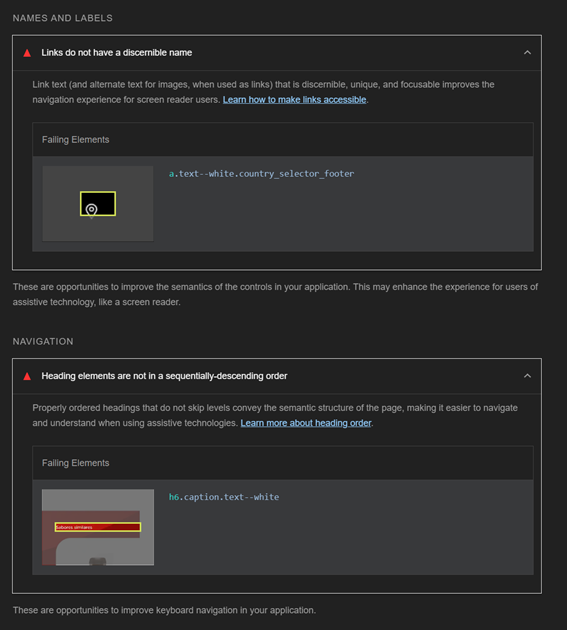
\includegraphics[width=0.25\linewidth]{Imagen6.png}
        \caption{Resultados análisis de www.nescafé.es}
\end{figure}

Además de los problemas mencionados anteriormente, la herramienta de análisis también detecta deficiencias relacionadas con las etiquetas de imágenes y el orden de los atributos en la página. Que tal y como ya explicamos en el análisis manual la existencia de estos errores contribuye a hacer que la página sea menos accesible y dificultan la comprensión y el uso eficiente de su contenido.

\newpage
\subsection{Wave:}

Además de utilizar Lightroom para el análisis de la página web, hemos llevado a cabo una evaluación adicional mediante la herramienta Wave. Esta doble revisión nos ha permitido obtener una perspectiva más completa y detallada de la accesibilidad del sitio.

\begin{figure}[!h] 
        \centering
        \includegraphics[width=1\linewidth]{Sin título2.png}
        \caption{Resultados análisis con Wave}
\end{figure}

En un principio Wave al igual que Lightroom encuentra errores en la robustez, al ver que le faltan varias etiquetas a la pagina web.

\begin{figure}[!h]
        \centering
        \includegraphics[width=0.25\linewidth]{Sin título.png}
        \caption{Links no accesibles de Nescafé}
\end{figure}


Además, hemos verificado y confirmar que efectivamente existen numerosas áreas de la página que no son accesibles mediante el uso exclusivo del teclado, corroborando así las conclusiones obtenidas durante nuestro análisis manual previo.


\newpage
\newpage
\newpage
\section{Análisis: Aplicación móvil: Instagram}
Se ha elegido la aplicación móvil de Instagram debido a que es una interfaz que no para de cambiar constantemente y las quejas sobre su dificultad no paran en cada actualización. Son muchos los usuarios que se han quejado sobre esto y por ello parece sensato hacer un análisis al respecto. De nuevo, se clasificarán los problemas según correspondan a uno de los cuatro estándares: perceptible, comprensible, operable y robustez.
\subsection{Perceptible}

\begin{itemize}
    \item Icono sin nombre en el inicio. En la pantalla de inicio se muestra el icono y se comunica que es de Meta, la compañía de Zuckerberg. Sin embargo, no se tiene un texto que comunique al usuario qué aplicación se está abriendo, lo que para los que usen un lector de pantalla para guiarse es un problema.
    \begin{figure}[!h]
        \centering
        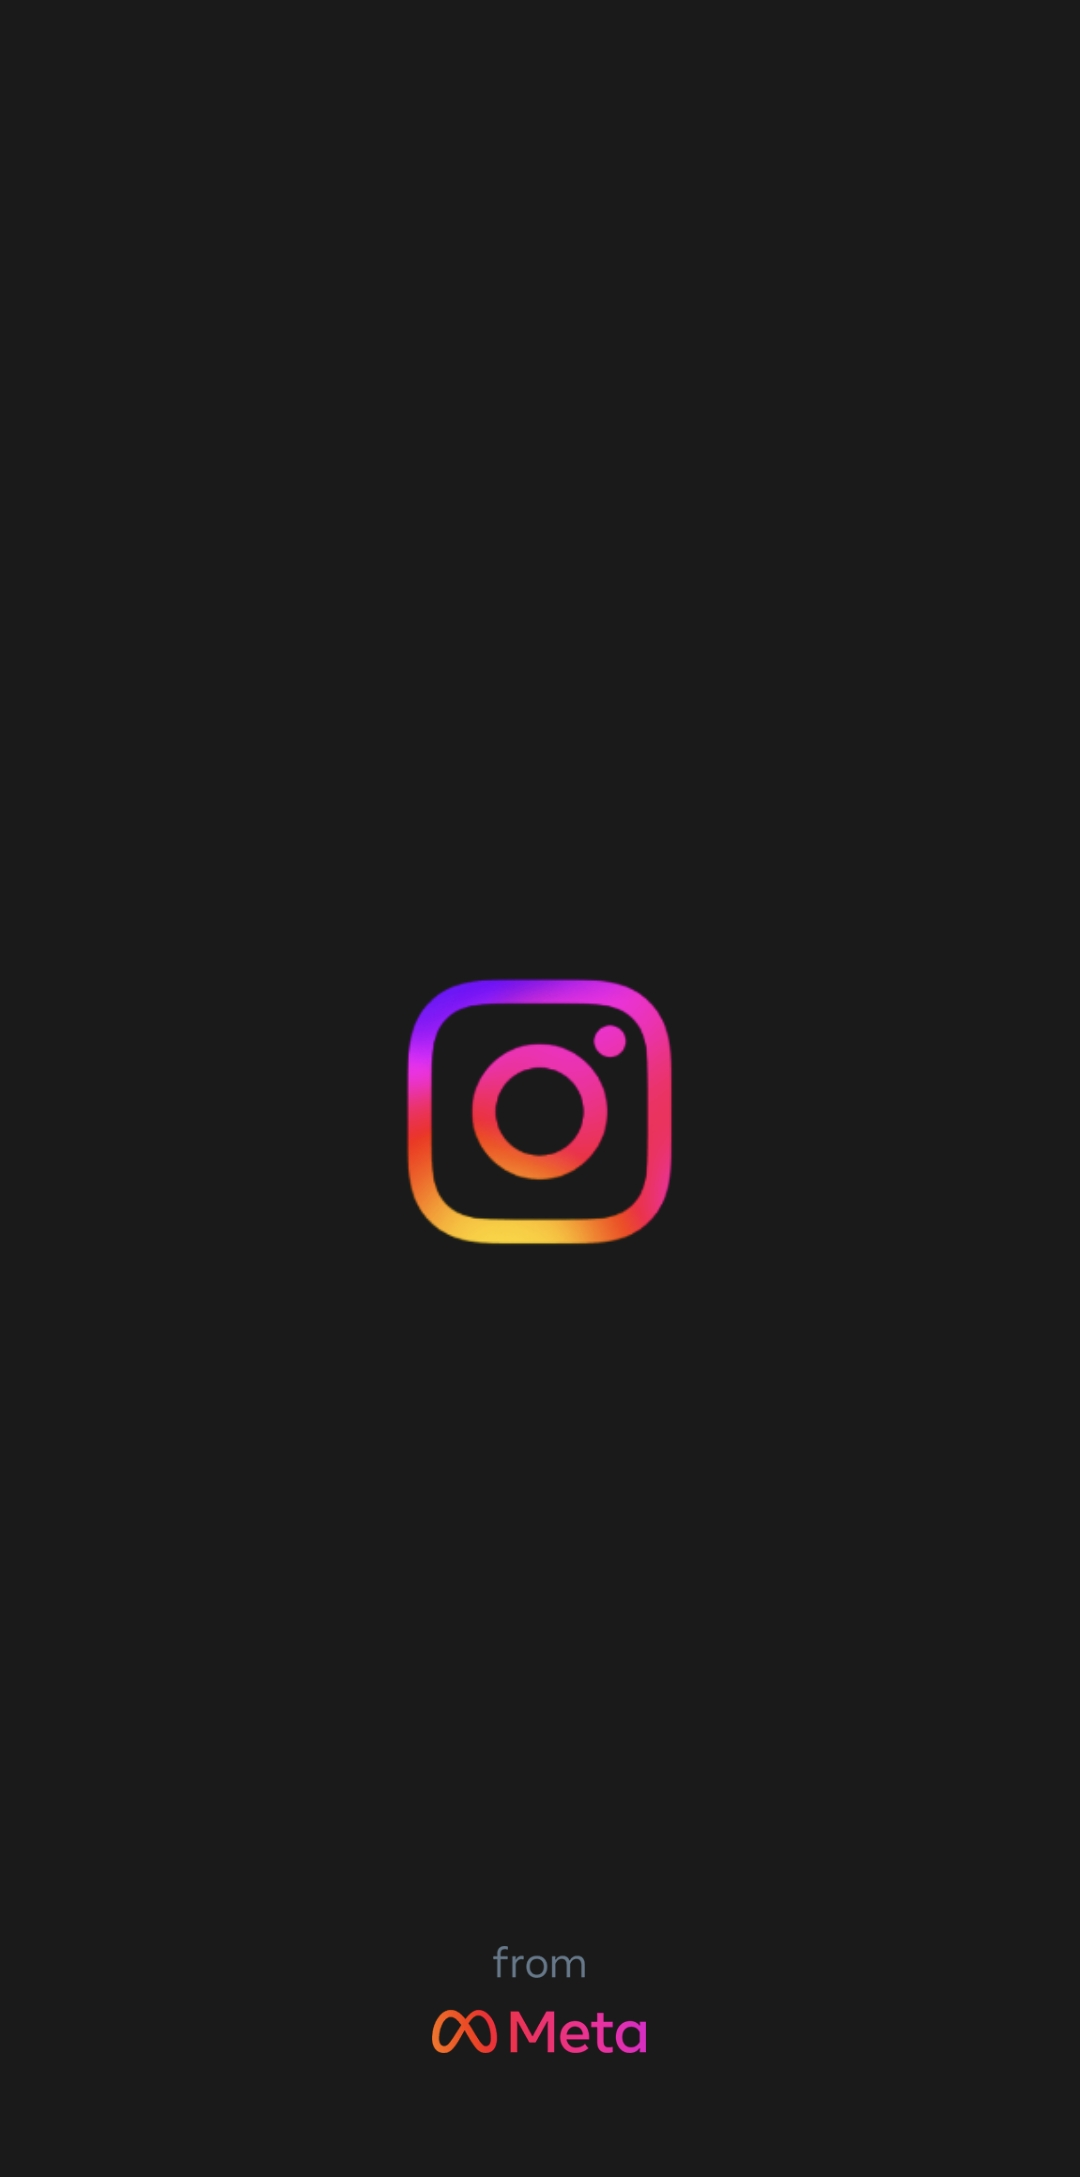
\includegraphics[width=0.20\linewidth]{img12.jpg}
        \caption{Icono de inicio de aplicación sin nombre}
    \end{figure}
    \item El modo oscuro está dentro del apartado de accesibilidad que se encuentra un poco oculto entre la gran cantidad de opciones. Lo positivo es que no es un icono o un toggle sin texto, sino que es una opción y dentro tiene cada opción con el nombre de “Activado”, “Desactivado” “Predeterminado del Sistema”. Esto ayuda a personas que estén utilizando un lector de pantalla y tengan problemas de visibilidad.
    \begin{figure}[!h]
        \centering
        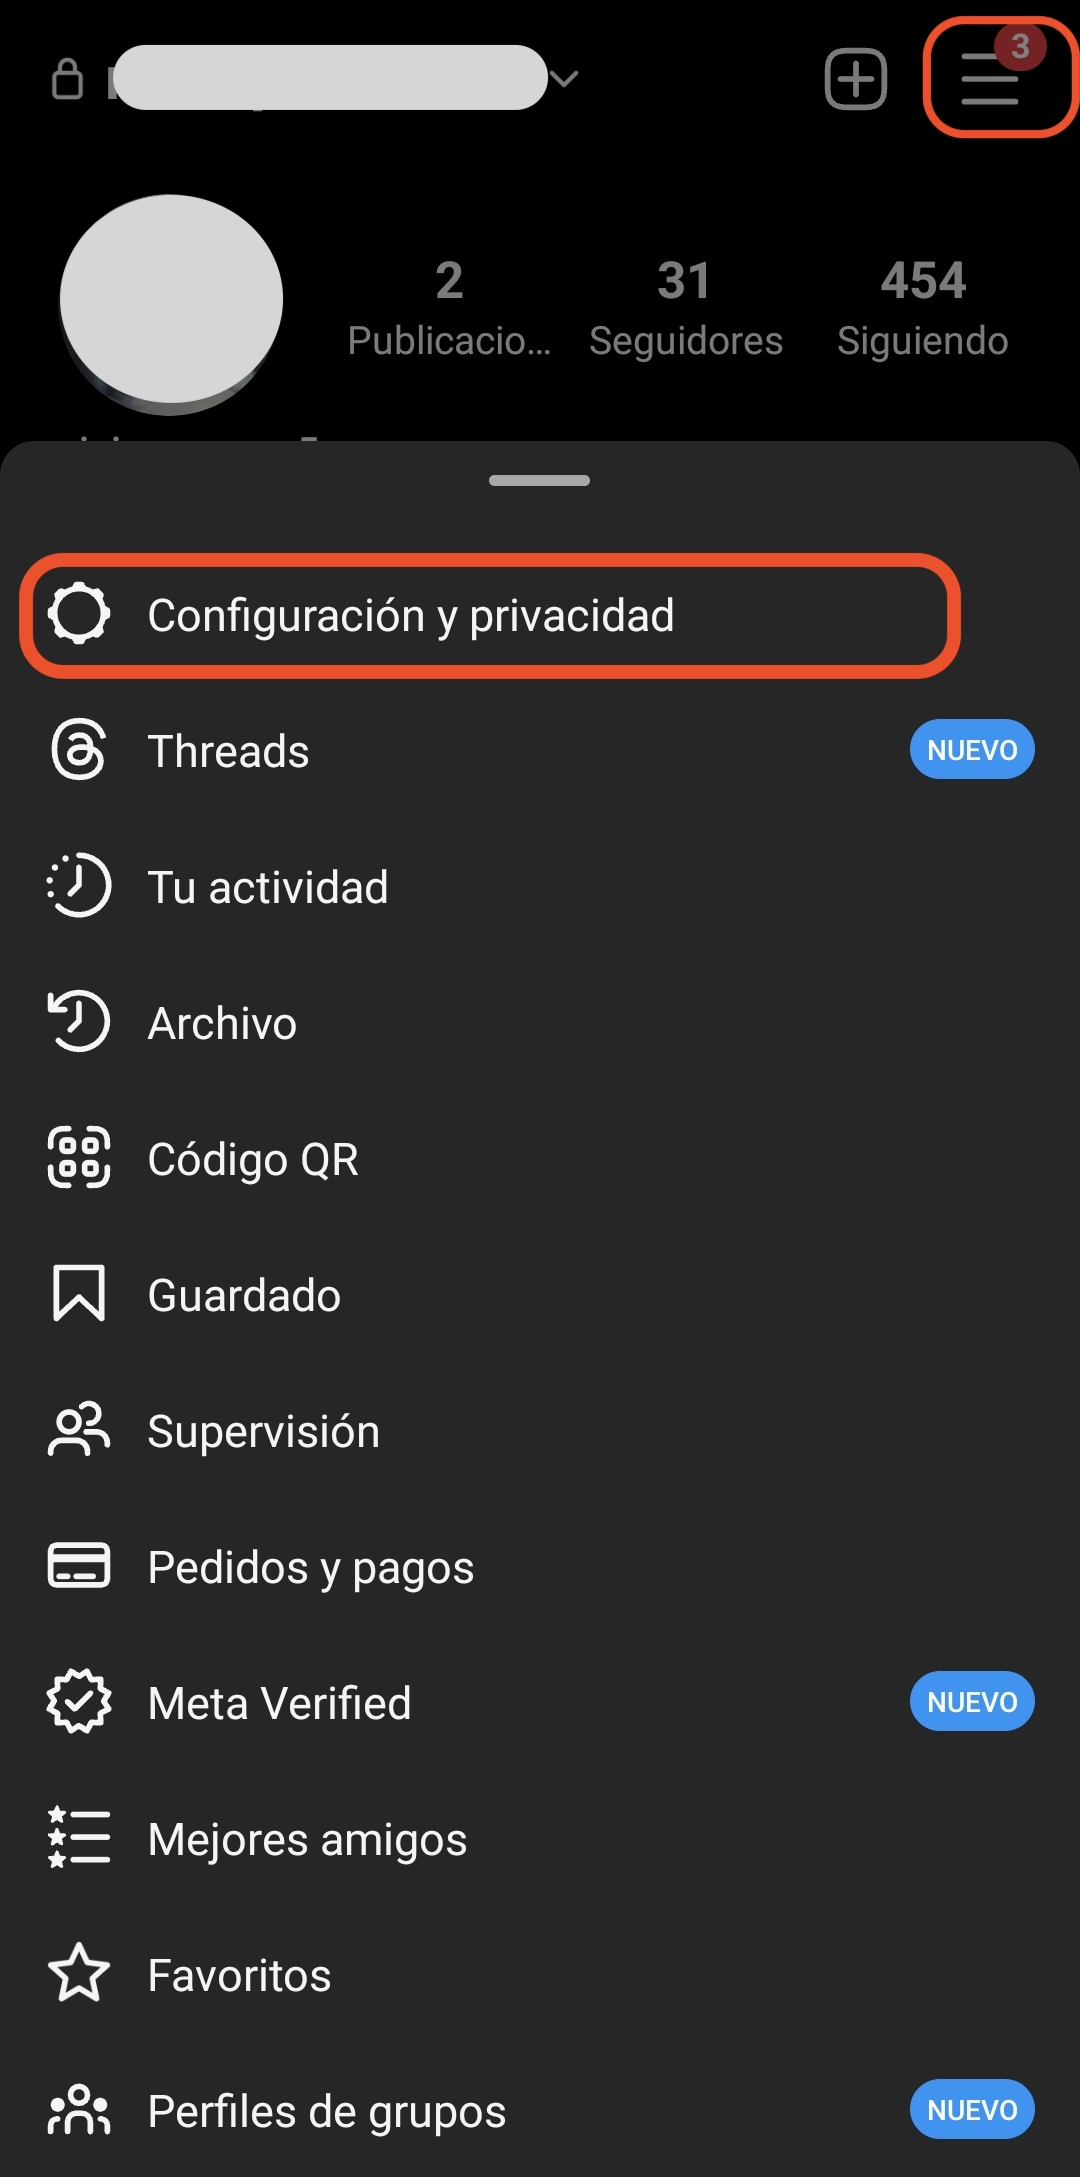
\includegraphics[width=0.20\linewidth]{img9.jpg}
        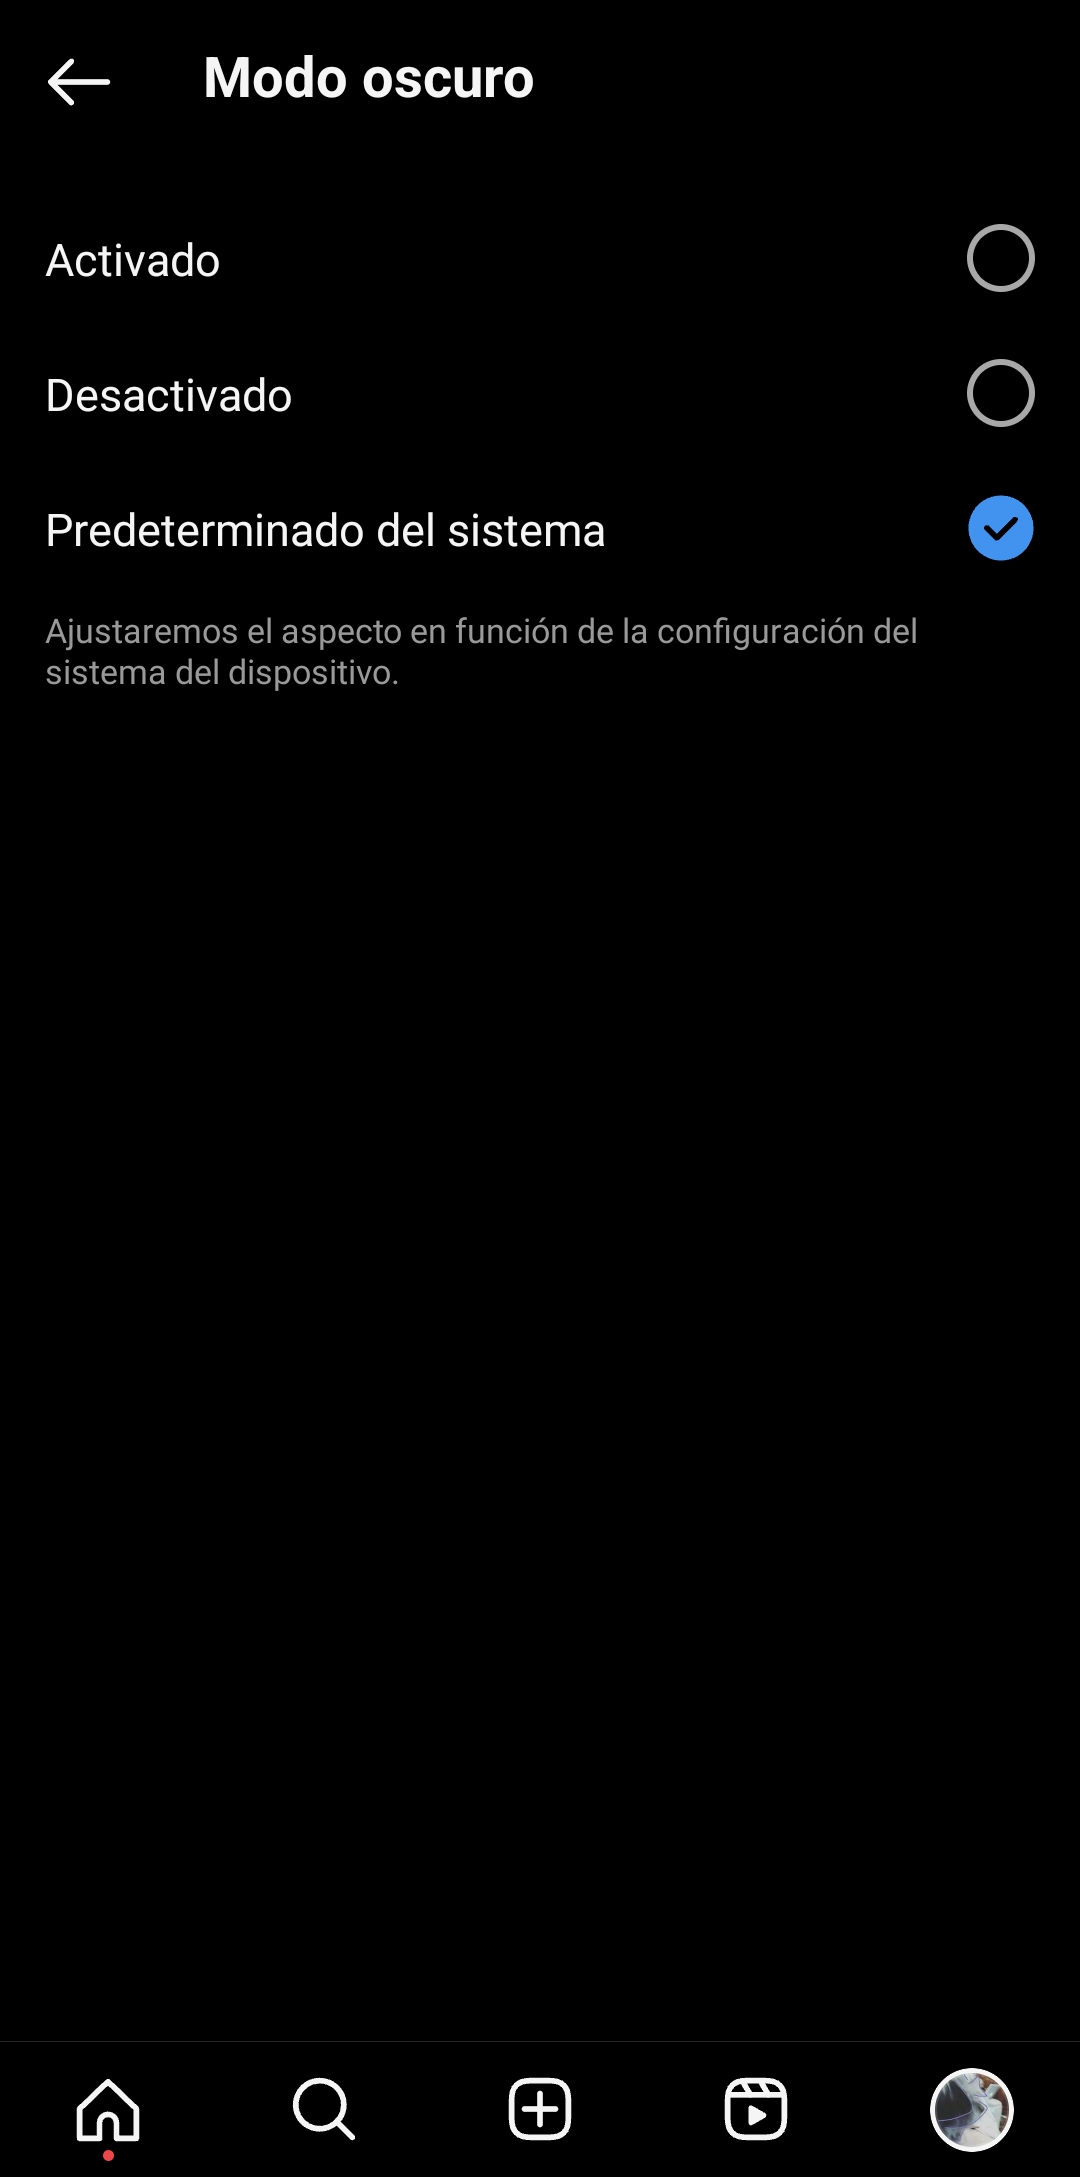
\includegraphics[width=0.20\linewidth]{img7.jpg}
        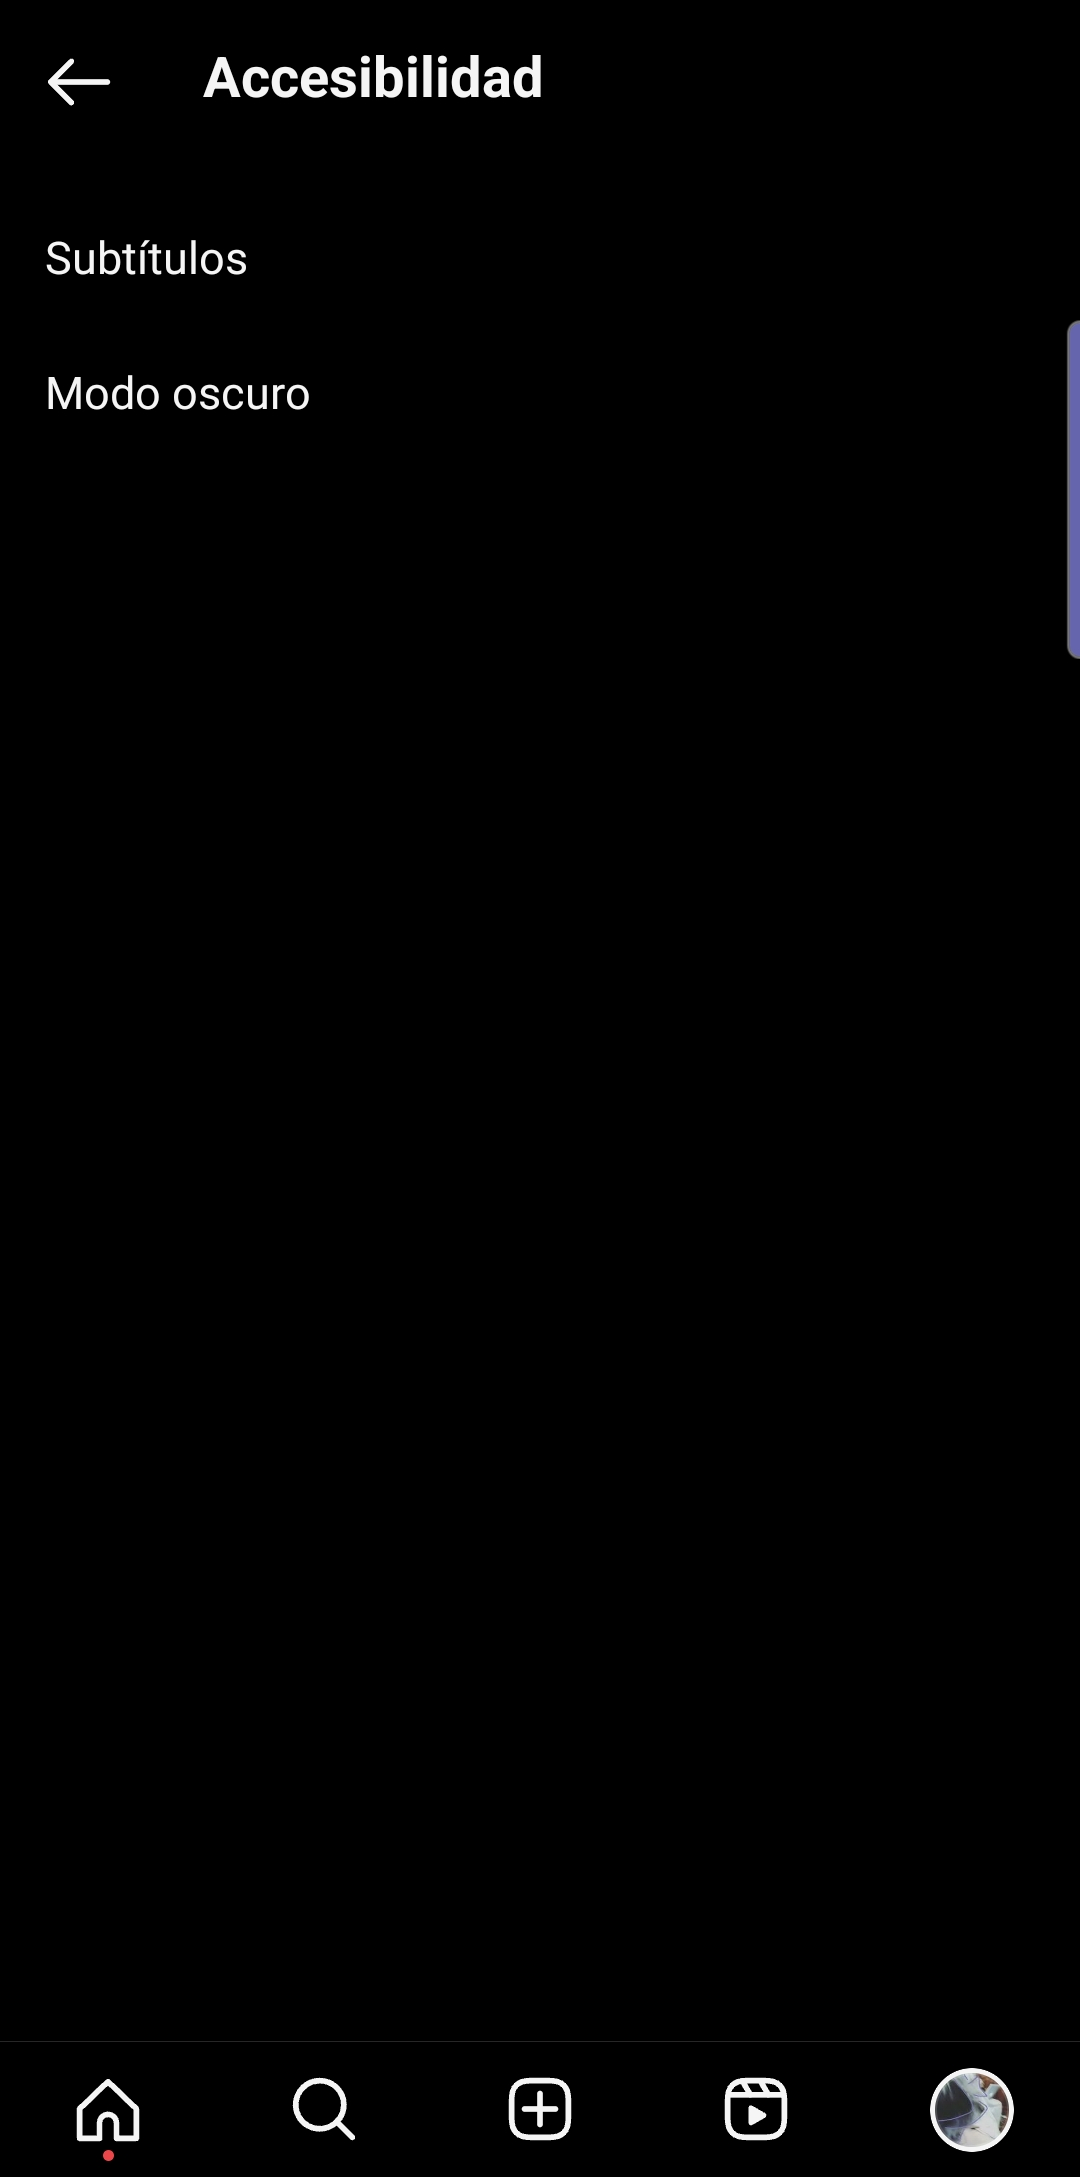
\includegraphics[width=0.20\linewidth]{img6.jpg}
        \caption{Modo oscuro difícil de encontrar}
    \end{figure}
    \item Espaciado: Algunos elementos de la interfaz de usuario están demasiado juntos, lo que puede dificultar que las personas con discapacidad visual los interactúen.
    \item Tamaño de fuente: El tamaño de fuente predeterminado es demasiado pequeño para algunas personas, lo que puede dificultar su lectura.
    \begin{figure}[!h]
        \centering
        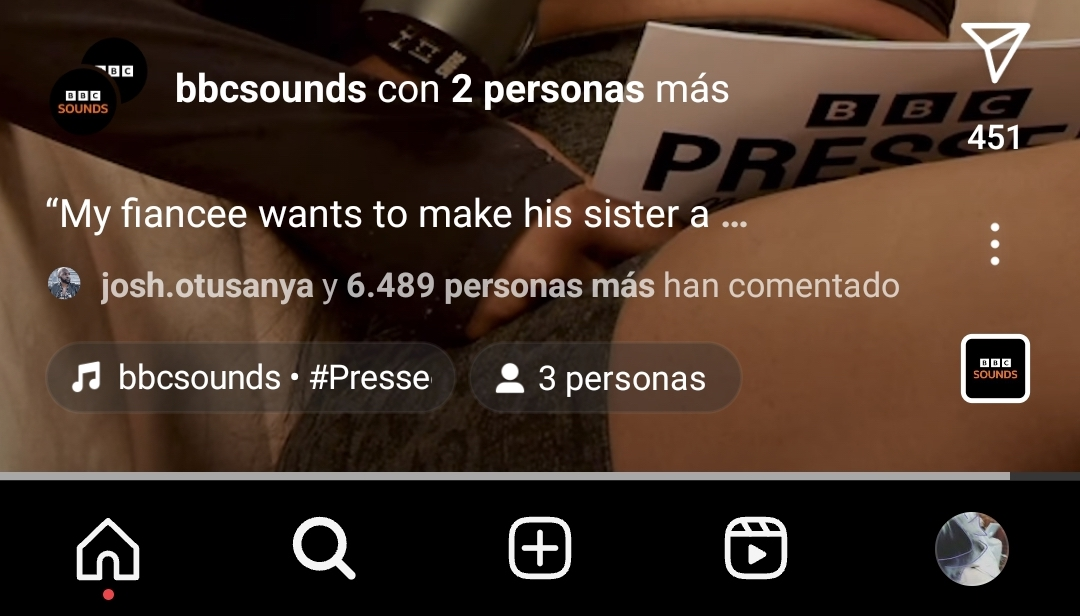
\includegraphics[width=0.20\linewidth]{img5.jpg}
        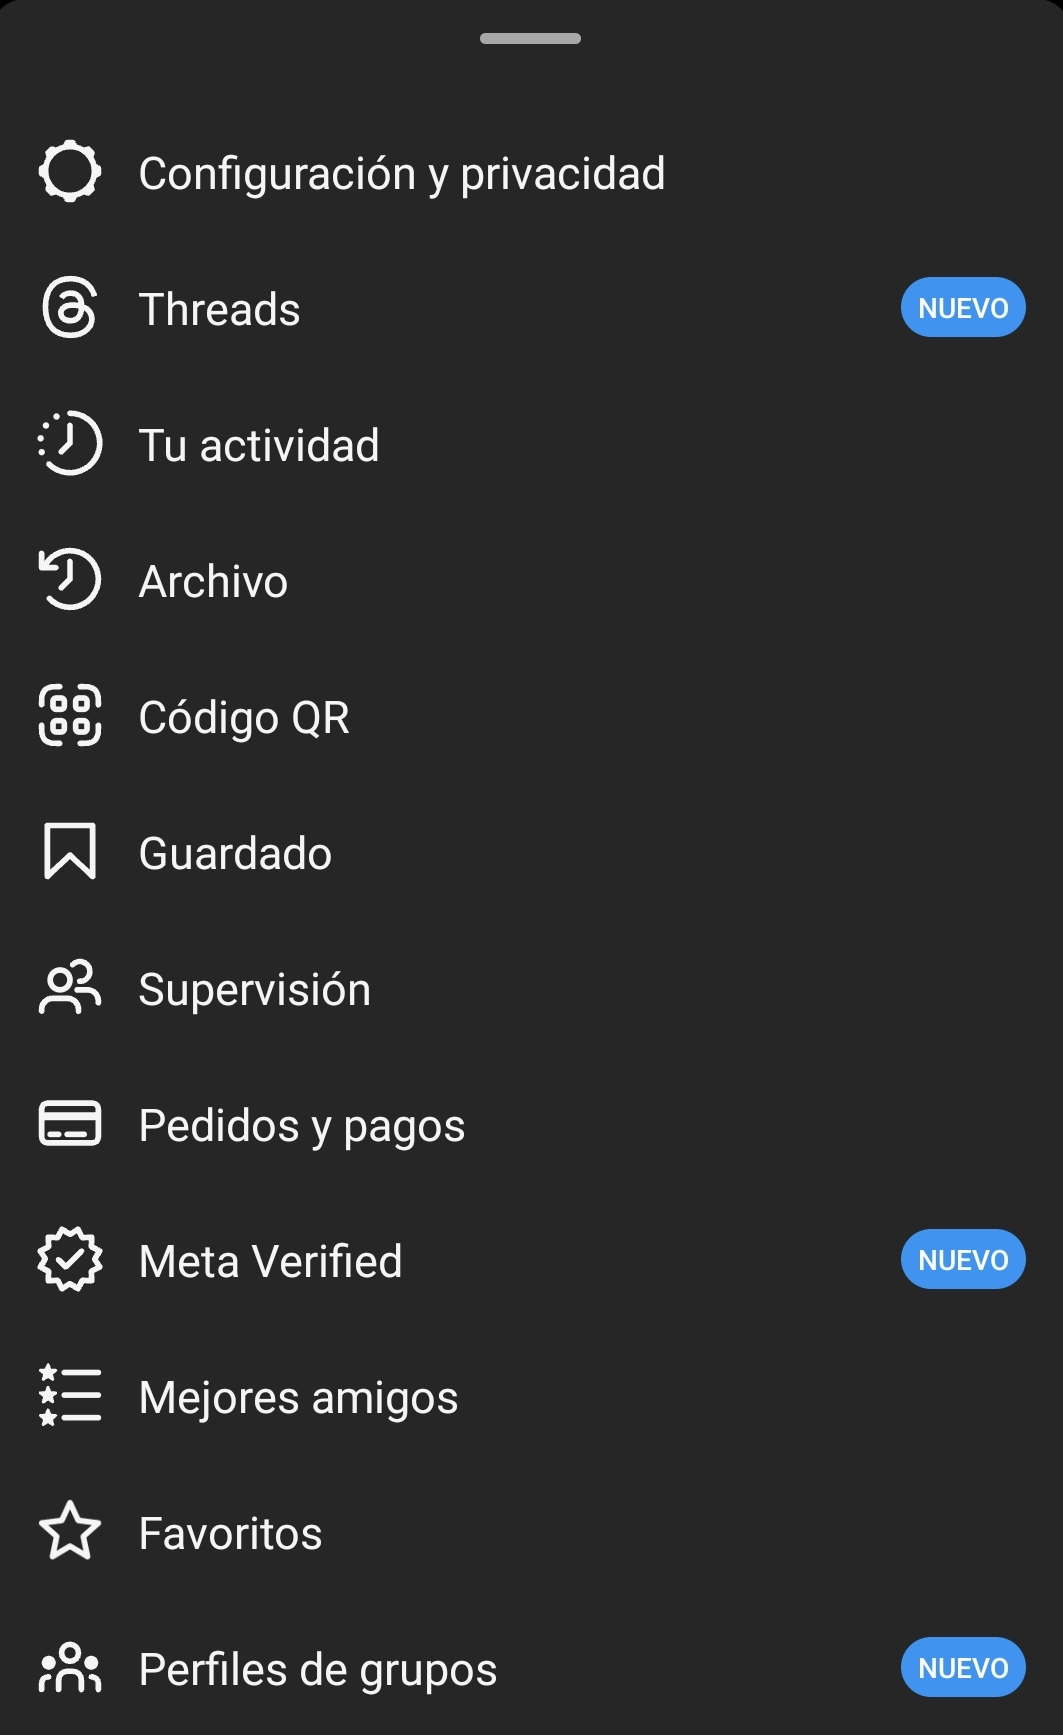
\includegraphics[width=0.20\linewidth]{img8.jpg}
        \caption{Espaciado escaso entre los elementos y fuente pequeña}
    \end{figure}
    
    \item Ruido visual: Las pantallas de los reels pueden estar muy llenas en ocasiones y molestar o impedir la lectura de subtítulos.
    \begin{figure}[!h]
        \centering
        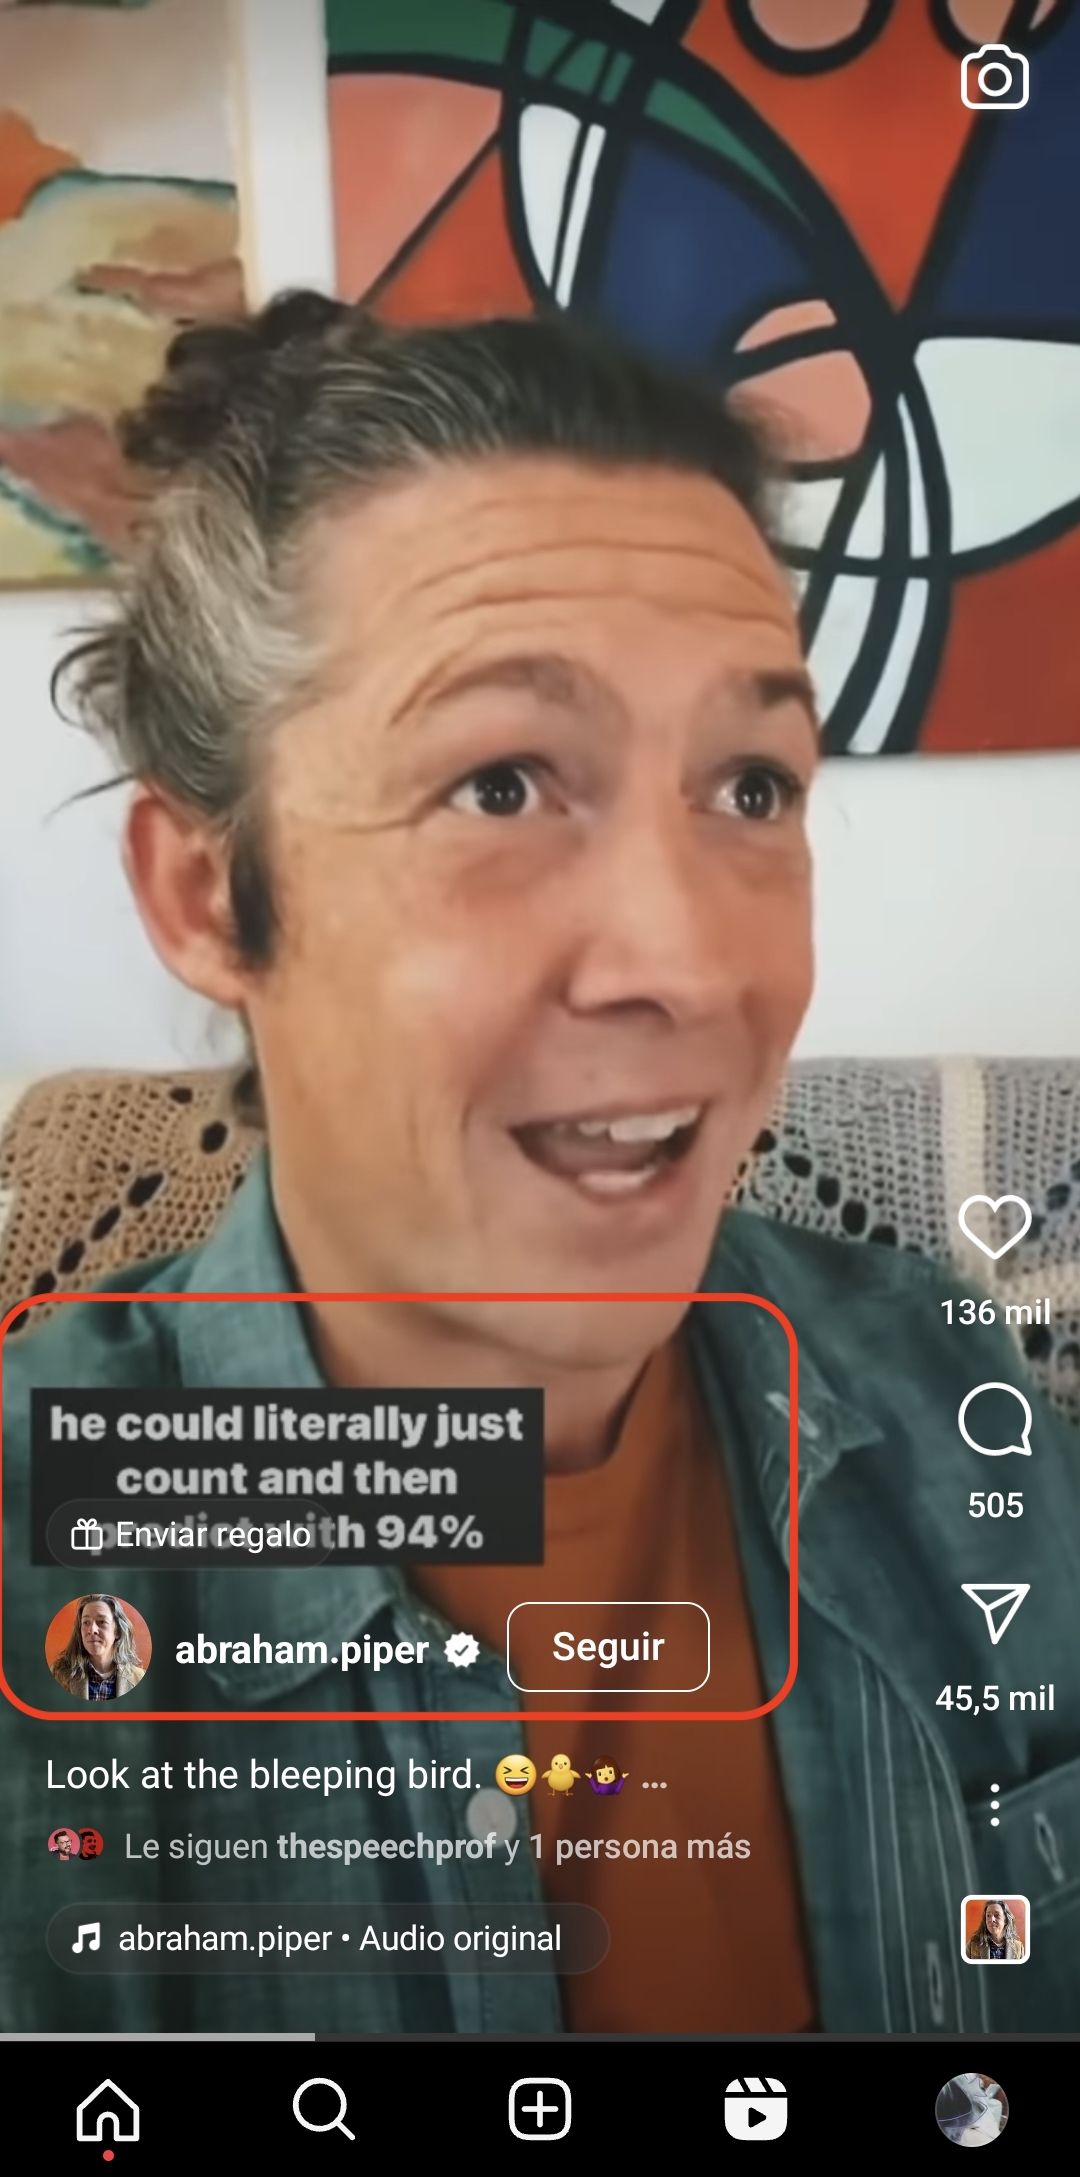
\includegraphics[width=0.20\linewidth]{img13.jpg}
        \caption{Impedimento de lectura de subtítulos}
    \end{figure}
    \item Falta de contrate en la letra. Una persona con discapacidad visual puede tener dificultades para leer el texto en la aplicación. El texto no tiene un contraste suficiente con el fondo, lo que puede dificultar su lectura. Esto afecta tanto al apartado de perceptibilidad como el operable, ya que muchos botones al ser siempre blancos, cuando el fondo del vídeo es del mismo color o muy claro, la letra no se lee bien. En el apartado de accesibilidad no hay opción para cambiar esto.
    \item Icono pequeños. Sobre todo en las descripciones largas, para leerlas por completo hay que hacer clic sobre los tres puntos suspensivos. Esto es un problema muchas veces y se acaba por clicar en la pantalla (y por lo tanto desactivar el audio del vídeo) antes que darle al icono. Y muchas veces no es muy visible por las razones dadas sobre el contraste anteriormente.
\newline
    \begin{figure}[!h]
        \centering
        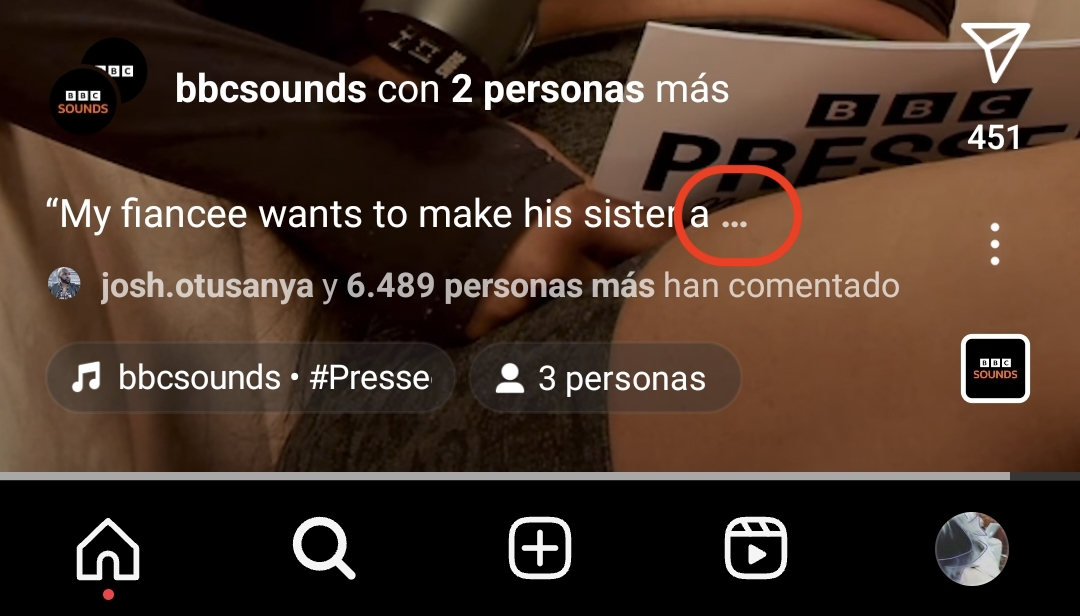
\includegraphics[width=0.20\linewidth]{img14.jpg}
        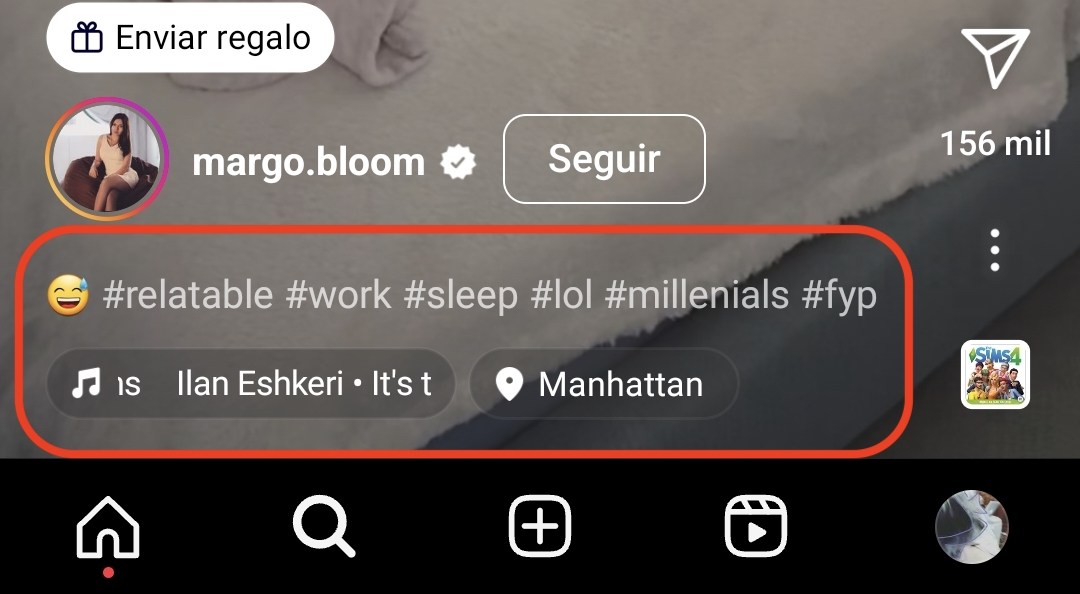
\includegraphics[width=0.20\linewidth]{img15.jpg}
        \caption{Letras con poco contraste y elementos demasiado pequeños para clicar}
    \end{figure}
    
\end{itemize}


\subsection{Comprensible}
\begin{itemize}
    \item Uso de un mismo icono para dos operaciones distintas. El icono 
\includegraphics[width=5mm]{3 puntos.png}
 en la barra inferior hace referencia a crear una historia, y te abre la cámara directamente. Mientras que en la página de perfil el mismo icono pero en la parte superior te lleva una lista donde eliges qué tipo de publicación se quiere crear.
    \begin{figure}[!h]
        \centering
        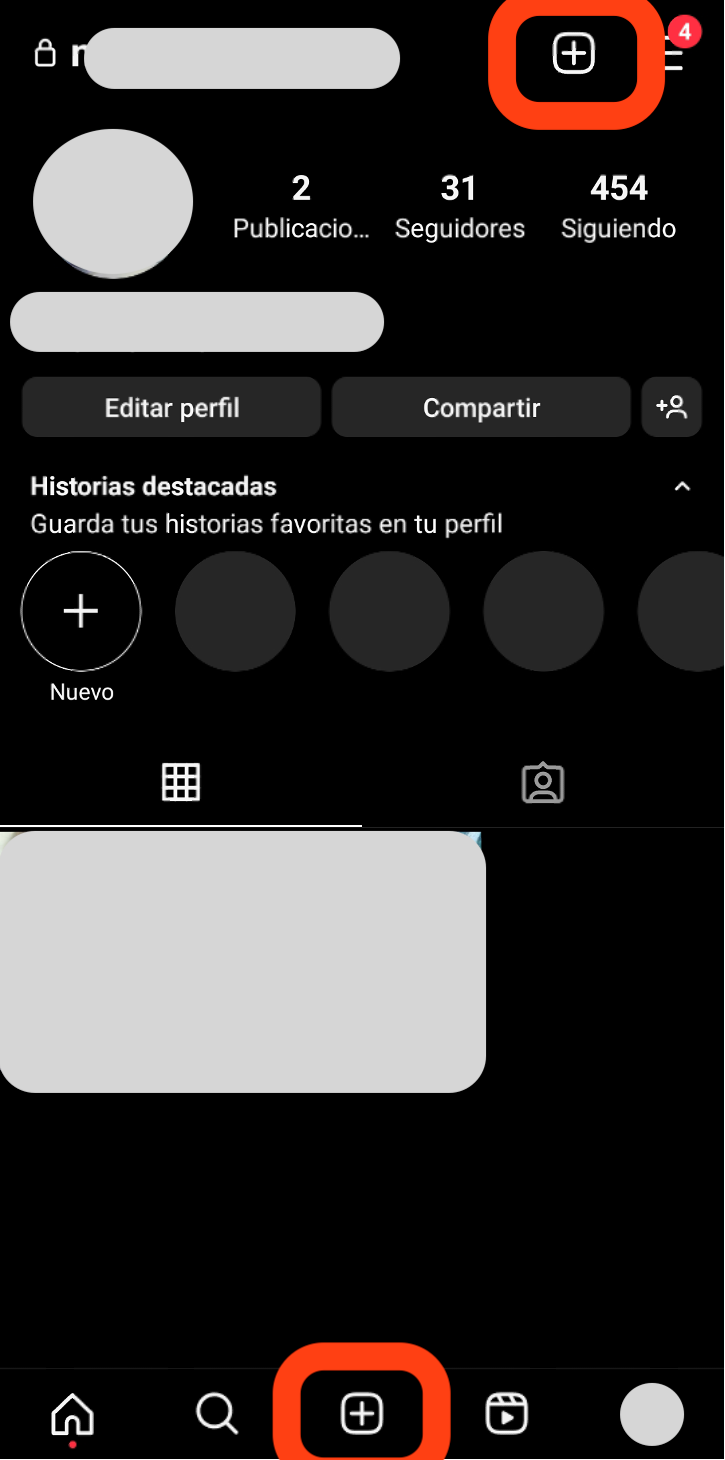
\includegraphics[width=0.20\linewidth]{img16.png}
        \caption{Mismo botón, distinta opción}
    \end{figure}
    \item También hay notificaciones en forma de círculo azul en la pestaña de mejores amigos. Sin embargo no tiene texto y cuando se pulsa la notificación no se muestra qué cambio hay en la lista. Simplemente es como si el usuario entrara aunque no hubiera notificación. Es decir, falta información para el usuario de por qué se le notifica de algo.
    \item La app tiene muchas pantallas con demasiadas opciones diferentes. Esto a un usuario experto, que se dedique a la creación de contenido puede serle útil, pero para el usuario promedio que sólo entra para ver contenido, tantas opciones resultan abrumadoras. Hay demasiadas pantallas con listas de acciones que no se utilizan con la suficiente frecuencia como para justificar sus disposición. Y esto no sólo molesta sino que dificulta encontrar aquellas opciones que sí se van a utilizar.
    \newline
\newline
\newline
\newline
\newline
\newline
\newline
\newline
\newline
\newline
    \begin{figure}[!h]
        \centering
        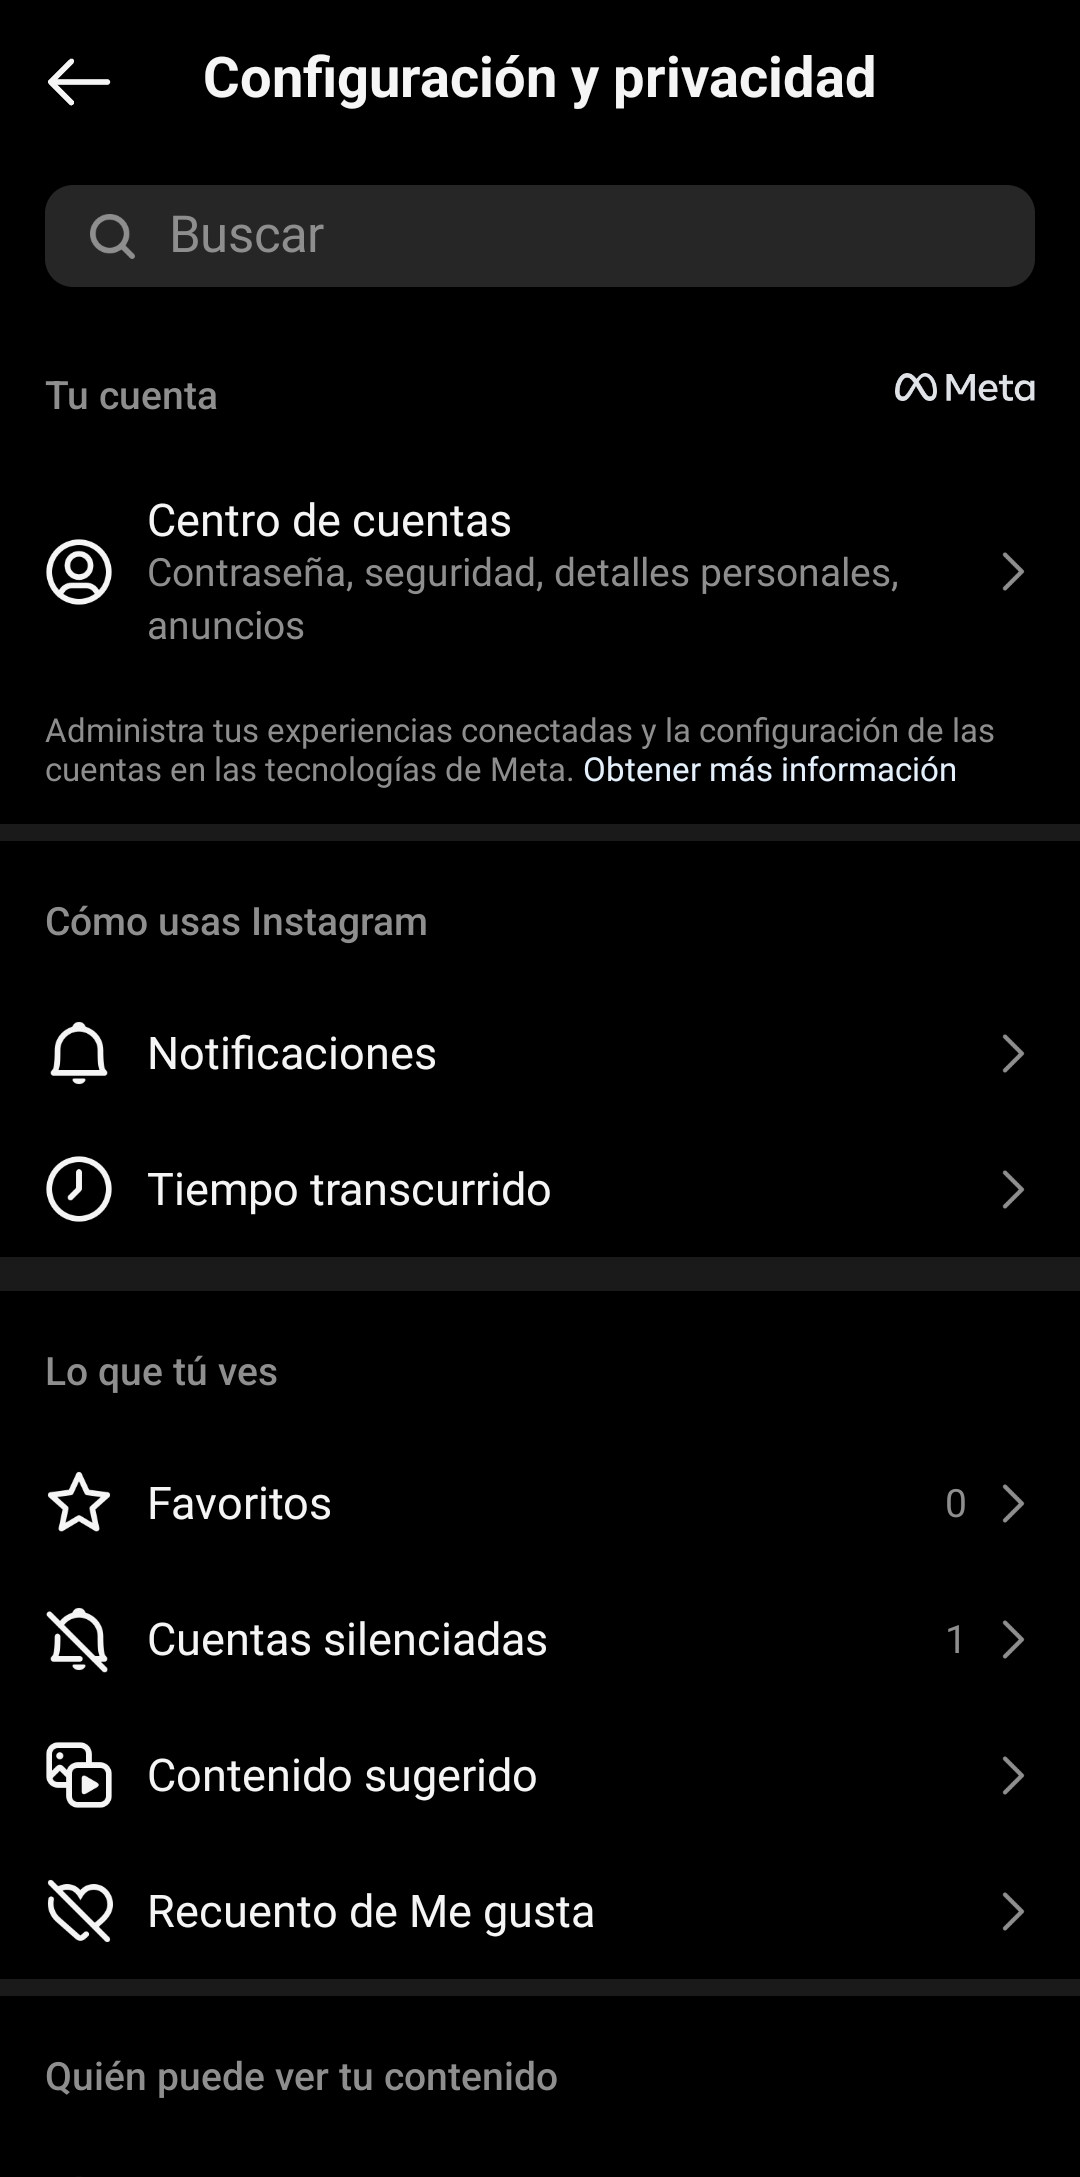
\includegraphics[width=0.20\linewidth]{img17.jpg}
        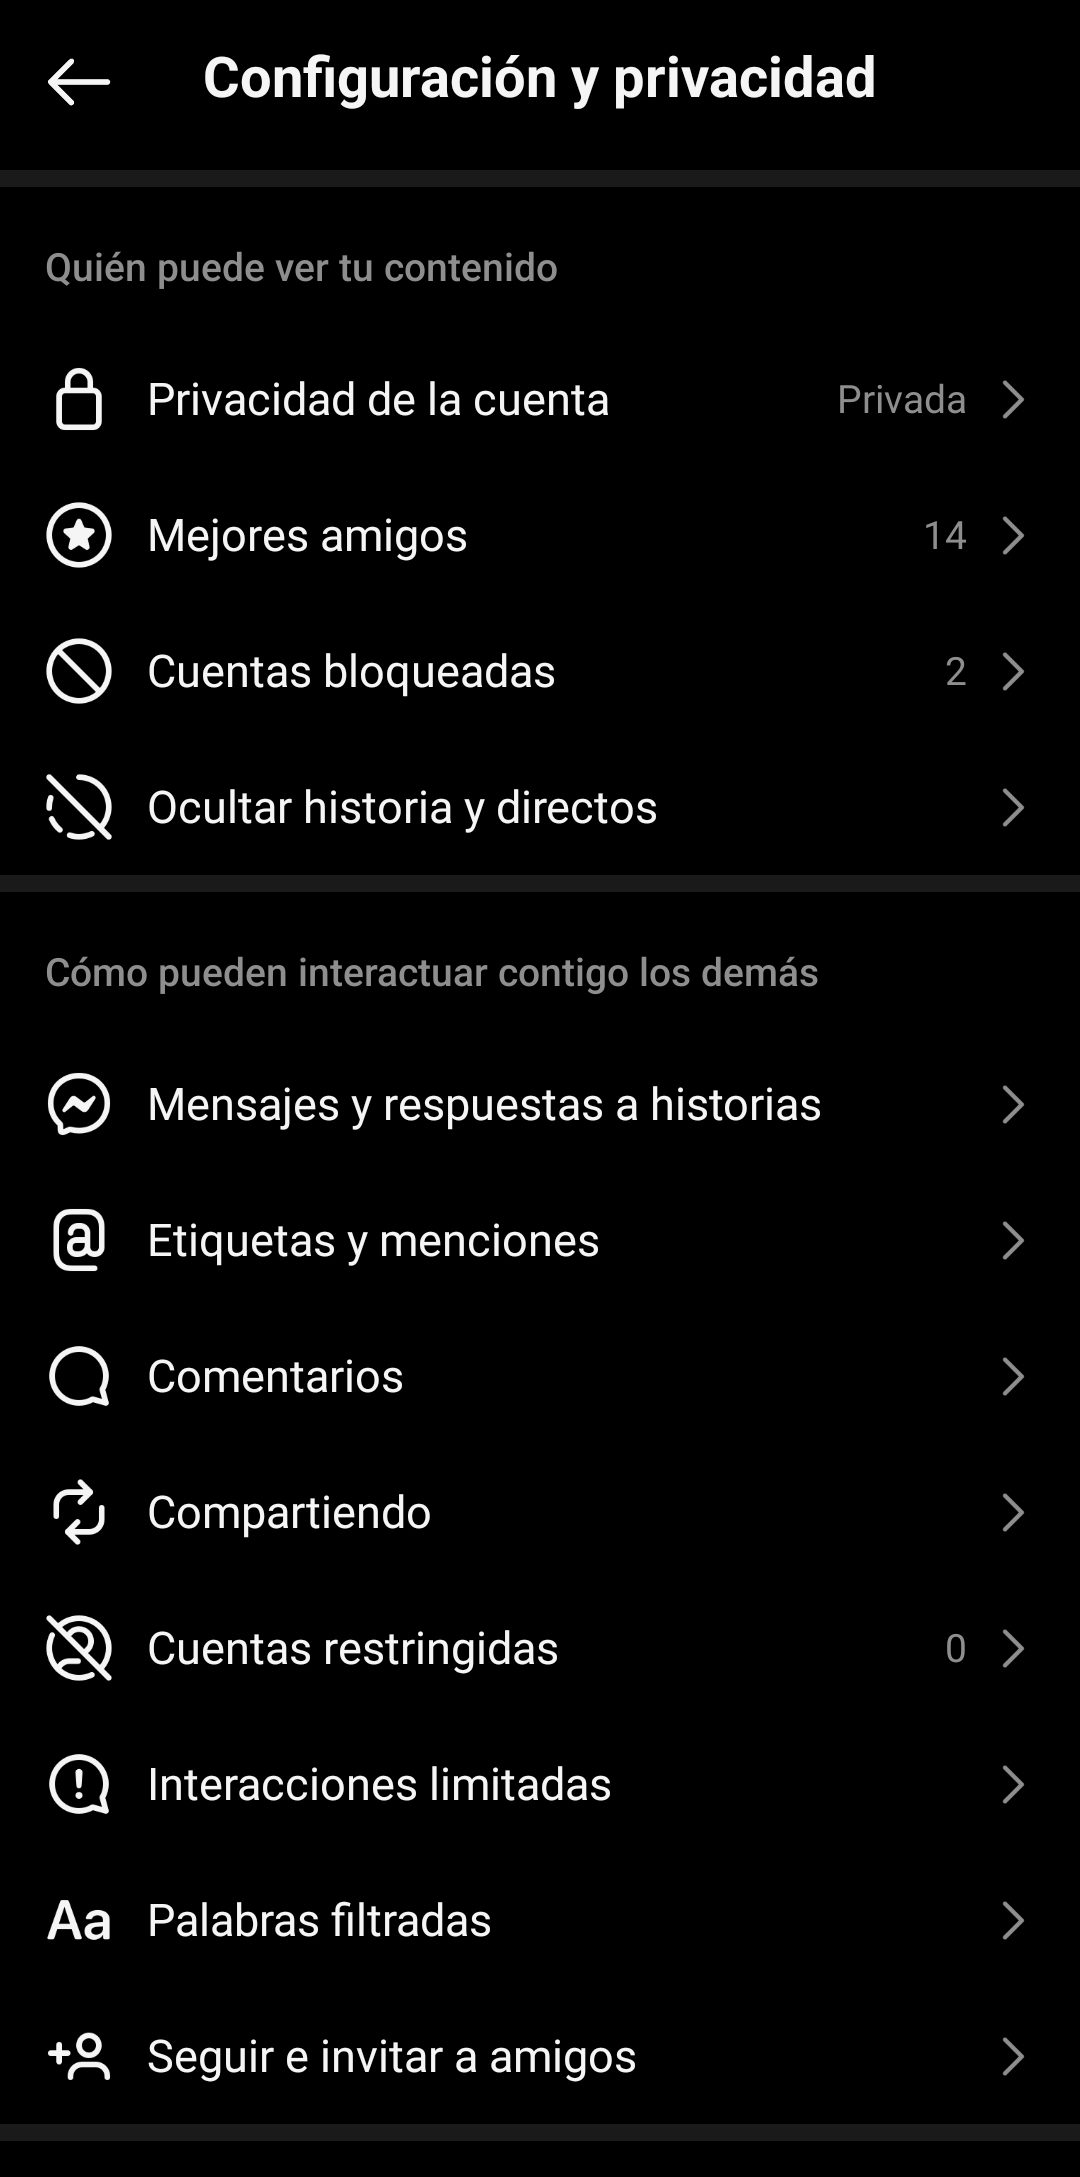
\includegraphics[width=0.20\linewidth]{img18.jpg}
        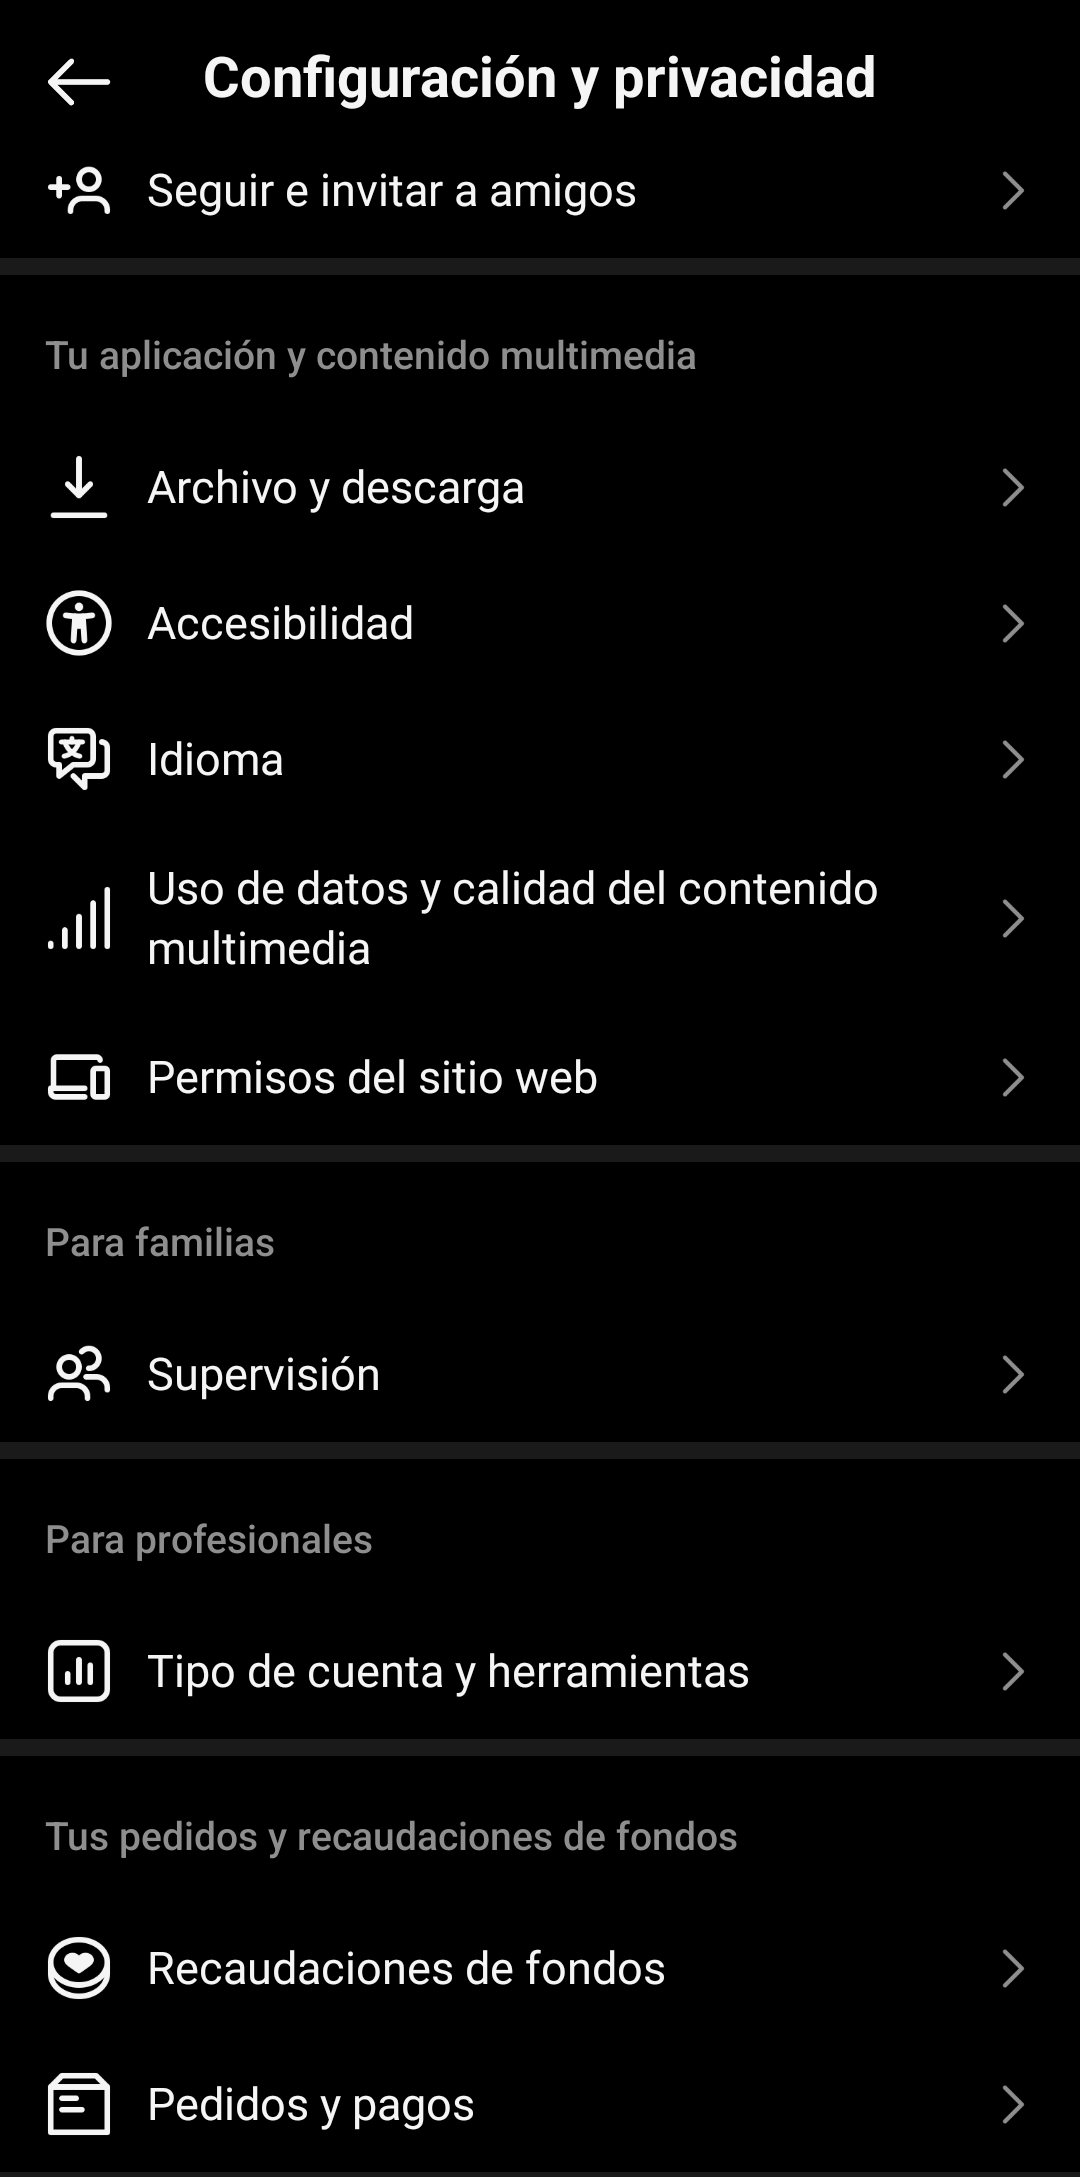
\includegraphics[width=0.20\linewidth]{img19.jpg}
        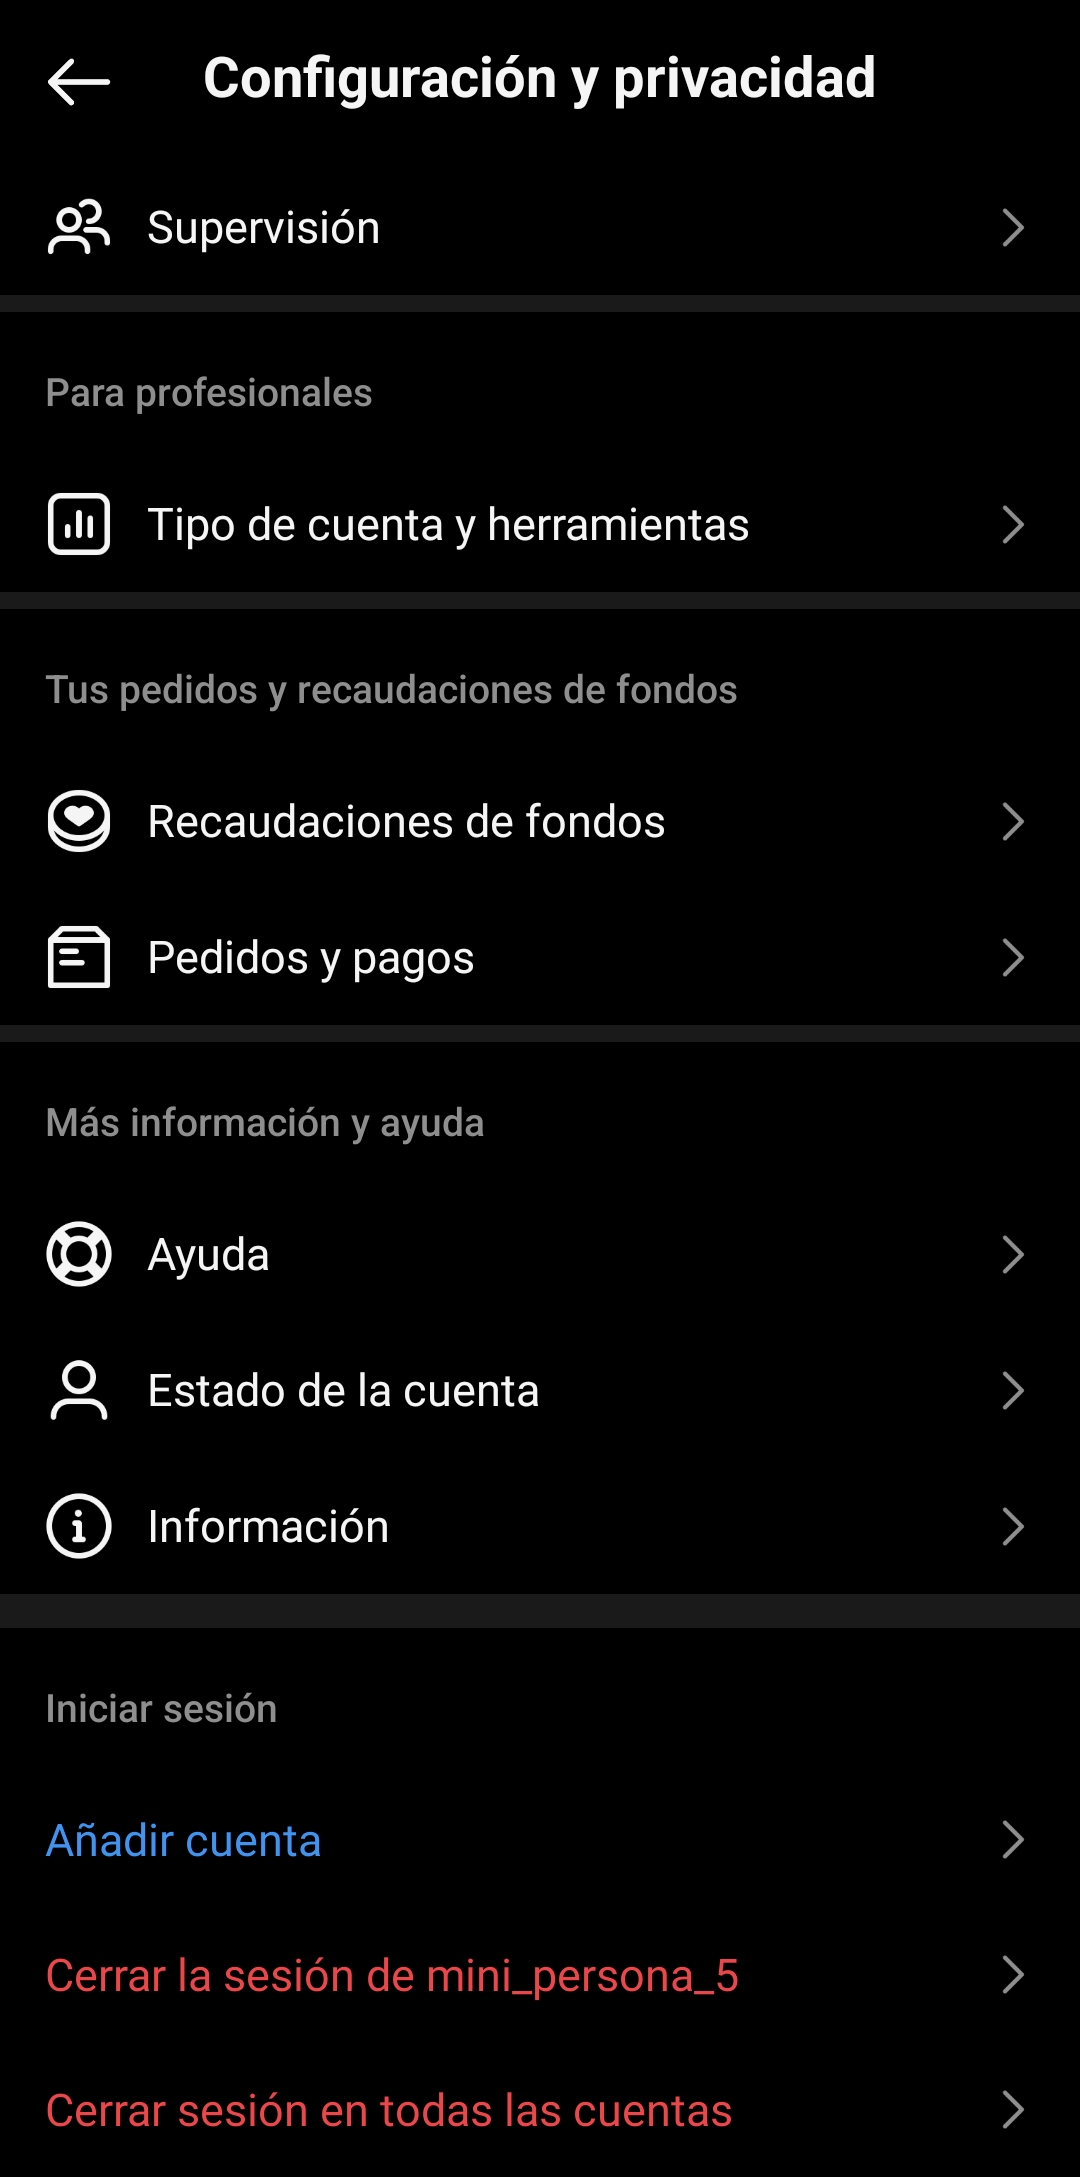
\includegraphics[width=0.20\linewidth]{img20.jpg}
        \caption{Imágenes de opciones en configuración general de la cuenta (además de las enseñadas en la figura 10.1)}
    \end{figure}
\end{itemize}



\subsection{Operable}

\begin{itemize}    
    \item Una persona con discapacidad cognitiva puede tener dificultades para aprender cómo usar la aplicación. La interfaz de usuario es compleja y tiene muchos menús y opciones.
    \item Los vídeos se paran manteniendo el dedo, cuando en TikTok y en YouTube Shorts se paran pulsando sobre la pantalla. Aquí no es solo problema de universalidad, sino que es menos práctico parar un vídeo teniendo que mantener el dedo, además de que añade un retardo desde que pulsas hasta que para el vídeo, y por lo tanto en vídeos que van muy rápido puede que no pare en el momento que tú indicas
\end{itemize}

\subsection{Robustez}
\begin{itemize}
    \item Una persona en un área con una conexión de red lenta puede tener dificultades para usar la aplicación. La aplicación puede ser lenta para cargar y puede tener problemas para funcionar correctamente.
    \begin{figure}[!h]
        \centering
        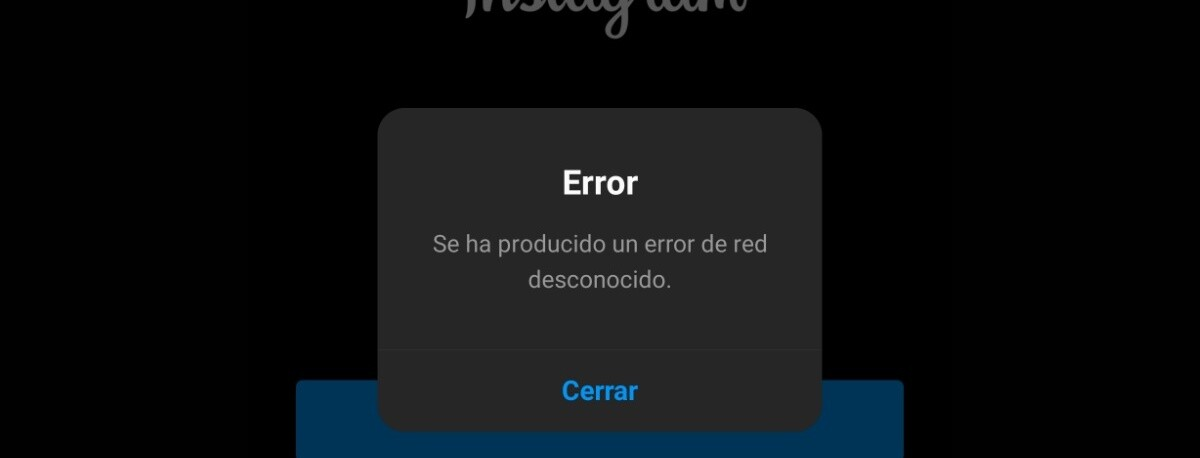
\includegraphics[width=0.30\linewidth]{img21.jpeg}
        \caption{Problemas con la conexión de red}
    \end{figure}
    \item Por lo general la app suele ser bastante robusta pero siempre hay posibilidad de errores inesperados que cierren la aplicación de pronto.
    \item Interrupción: La aplicación puede interrumpirse debido a problemas de red o problemas del dispositivo. Normalmente, cuando se cambia de aplicación y se deja Instagram en segundo plano durante más de 30 segundos y luego se vuelve a poner en primer plano, el que se estaba reproduciendo reel empieza desde el principio. O si estamos en un feed, puede recargar el feed desde el principio o uno completamente distinto, y se pierden los posts que estabas viendo.
    \item Se suelen notar más fallos en la versión de Android.
    
\end{itemize}

\section{Anexo}
El trabajo se encuentra en el siguiente link: \href{https://github.com/MinervaQuin/Accessibility-Report.git}{https://github.com/MinervaQuin/Accessibility-Report.git}




\end{document}